\section{Реализация}
\label{sec:implementation}

В этом разделе наше внимание сместится на осбенности реализации процессов
связанных с типами в Scala Plugin и особенности их инструментирования.
\textbf{Так как конечной целью является визуализация работы этих процессов, то
хочется максимально опираться на стандарт языка, которым является спецификация
scala \cite{scala_spec}.}
Мы проследим как соответсвующие понятия из спецификации переносятся в Scala Plugin.
А там где это не возможно будет явно указано на расхождение в реализации плагина и
спецификации.
Так-же будет указано как визуализируется каждый процесс.

% Реализация в плагине в плагине
% Смысл в последующей визуализации
% Хочется сделать С уважением к спецификации
% Однако не везде это возможно сделать
% Где можно сделаем
% Везде будет указано расхождение

До этого момента, когда мы говорили о работе плагина, то использовали
нейтральное слово процесс.
Теперь нужно вспомнить, что изначальной задачей было явно визуализировать
работу связанную с типами, которую плагин делает неявно.
Архитектура части плагина связанной с типами будет
рассмотрена в разделе \ref{sec:arch}.
Перечислим интересующие нас процессы.

Базовым процессом является сравнение двух типов.
В спецификации для этого вводятся три понятия: эквивалентность типов, сводимость
типов и слабая сводимость типов.
Эквивалентность означает что один тип мы в любом контексте можем заменить другим
типом, и это отношение наиболее понятно интуитивно.
Сводимость типов намного более интересна и используется во всех других процессах.
Ее мы рассмотрим в разделе~\ref{sec:conformance}.
Там же будет описание слабой сводимости, а также будет разобрано представление
типов в Scala Plugin и их отличия от типов описанных в спецификации scala.

Следующим интересующим нас процессом будет вывод типов.
Важно что вывод типов в плагине и в спецификации осуществляется по разному.
Подробно об этом будет написано в разделе~\ref{sec:infer}

Последний процесс, следующий из вывода типов - это разрешение перегрузок функций.
Действительно, типовые переменные появляются в вызовах полиморфных
функций и их неявный вывод актуален для конкретного вызова.
А так как в scala присутствуют перегрузки функций, то прежде всего нужно
разрешить символ на котором были вызваны аргументы.
Процесс разрешения перегрузок будет рассмотрен в разделе~\ref{sec:overloading}.

Отдельного упоминания заслуживает механизм implicit.
В данной работе не затрагивались неявные преобразования и неявные параметры.
В рамках Scala Plugin уже существуют ShowImplicitParametersAction, показывающий
неявно передаваемые параметры, и GoToImplicitConversationAction, помогающий
в работе с неявными преобразованиями.
Так же в данной работе не освященна работа с динамическими типами.

\subsection{Архитектура Scala Plugin}
\label{sec:arch}

\begin{figure}[t]
\centering
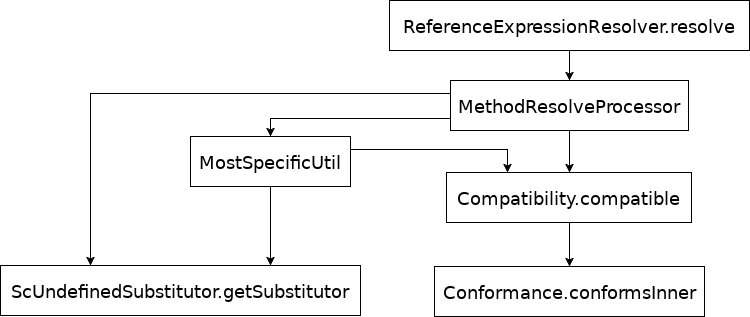
\includegraphics[width=\textwidth]{img/call-graph}
\caption{Граф вызовов}
\label{fig:callGraph}
\end{figure}

Как говорилось в начале главы~\ref{sec:implementation}, нас будут интересовать
процессы сведения типов, выведения типов и выбора перегрузки функции.
Все эти процессы можно проилюстрировать на вызове полиморфной функции.
Для начала рассмотрим как он будет обрабатываться плагином с
точки зрения архитектуры.
На рисунке~\ref{fig:callGraph}, несколько упрощенно, показан граф вызовов
такой обработки.
Мы явно будем указывать классы, основные и вспомогательные функции в которых
использовалась аннотация uninstrumented.
Это нужно чтобы понять куда именно добавлялась инструментация.
% основываясь на интересующих нас процессах

\textbf{Улучшить введение.}
Представим что у нас есть символ \textbf{f} и аргументы
\textbf{e1} ,..., \textbf{en}.
Для проверки этого применения будет вызван метод \textbf{resolve} объекта
\textbf{ReferenceExpressionResolver}.
Это и будет точкой входа.
Аннотировано uninstrumented:
\begin{itemize}
  \item \textbf{ReferenceExpressionResolver.resolve}
\end{itemize}
% Здесь только к методу \textbf{resolve} будет добавлена аннотация uninstrumented.

Далее с помощью класса \textbf{MethodResolveProcessor} будет осуществлен
поиск кандидатов обладающих таким же именем как \textbf{f}.
\textbf{MethodResolveProcessor} будет хранить множество кандидатов и
результаты применения соответсвующих кандидатов к аргументам.
Также там находится часть логики по фильтрации кандидатов, более подробно о которой
будет написано в разделе~\ref{sec:overloading}.
Аннотировано uninstrumented:
\begin{itemize}
  \item класс \textbf{MethodResolveProcessor}
  \item \textbf{MethodResolveProcessor.problemsFor}
  \item \textbf{MethodResolveProcessor.candidates}
\end{itemize}
% Аннотация uninstrumented была добавлена к самому классу
% \textbf{MethodResolveProcessor}, а также к вспомогательным методам
% объекта-компаньона \textbf{problemsFor} и \textbf{candidates}.

Для каждого кандидата нужно проверить, возможно ли вызвать его с такими аргументами.
Инструменты для этого находятся в классе \textbf{Compatibility}.
Омновная часть кода здесь - это перебор разных конструкций Scala Plugin,
описывающих исходный код, а также способов применения к ним аргументов.
Например, разбор таких случаев как передача аргумента по имени или параметры со
значением по умолчанию.
Аннотировано uninstrumented:
\begin{itemize}
  \item \textbf{Compatibility.checkConformance}
  \item \textbf{Compatibility.checkConformanceExt}
  \item \textbf{Compatibility.compatible}
\end{itemize}
% Здесь аннотация uninstrumented добавлена к методам объекта
% \textbf{checkConformance}, \textbf{checkConformanceExt} и \textbf{compatible}.

Для проверки двух типов используется интерфейс \textbf{Conformance}.
У этого интерфейса две реализации: одна для системы типов scala, другая для
системы типов dotty \cite{dotty}, нового поколения языка scala.
В обоих случаях метод \textbf{conformsInner} возвращает пару: возможна ли
сходимость и набор ограничений на абстрактные типы при которых сходимость
возможна.
Про процесс сходимости написано в разделе~\ref{sec:conformance}.
Аннотировано uninstrumented:
\begin{itemize}
  \item \textbf{Conformance.conformsInner}
  \item \textbf{Conformance.computable}
  \item \textbf{Conformance.checkParameterizedTypes}
  \item \textbf{Conformance.addParam}
  \item \textbf{Conformance.addArgedBound}
  \item класс \textbf{Conformance.LeftConformanceVisitor}
\end{itemize}
% Здесь аннотации uninstrumented применяются к методам
% \textbf{conformsInner}, \textbf{computable}, \textbf{checkParameterizedTypes},
% \textbf{addParam}, \textbf{addArgedBound}, а также к
% классу \textbf{LeftConformanceVisitor}.

Далее необходимо проверить что ограничения полученные на предыдущем шаге
возможно разрешить.
Для этого есть интерфейс \textbf{ScUndefinedSubstitutor}.
Его реализуют \textbf{ScUndefinedSubstitutorImpl} и
\textbf{ScMultiUndefinedSubstitutor}.
Отличие одной реализации от другой состоит в том, что
\textbf{ScUndefinedSubstitutorImpl} хранит только один набор ограничений, в
то время как \textbf{ScMultiUndefinedSubstitutor} хранит сразу несколько.
Это может понадобится если существует более одного способа добиться сводимости
типов. Конкретно это используется для составных типов.
Заметим, что разрешение ограничений на абстрактные типы - это и есть вывод типов.
Больше информации можно получить в разделе~\ref{sec:infer} о выводе типов.
Аннотировано uninstrumented:
\begin{itemize}
  \item \textbf{ScUndefinedSubstitutor.addLower}
  \item \textbf{ScUndefinedSubstitutor.addUpper}
  \item \textbf{ScUndefinedSubstitutor.getSubstitutorWithBounds}
  \item \textbf{ScUndefinedSubstitutor.getSubstitutor}
\end{itemize}
% Аннотация uninstrumented используется методах \textbf{addLower},
% \textbf{addUpper}, \textbf{getSubstitutorWithBounds}, а также \textbf{getSubstitutor}.

Интересно заметить, что пара \textbf{Compatibility} и
\textbf{ScUndefinedSubstitutor} образуют что-то вроде алгоритма
Хиндли-Милнера \cite{hindley–milner}.

Остался класс \textbf{MostSpecificUtil}.
Он нужен если после всех проверок сделанных \textbf{MethodResolveProcessor}
осталось больше одного кандитата.
В таком случае требуется найти наиболее специфичного кандитата.
Именно этим \textbf{MostSpecificUtil} и занимается.
Подробнее в разделе~\ref{sec:overloading}.
Аннотировано uninstrumented:
\begin{itemize}
  \item класс \textbf{MostSpecificUtil}.
\end{itemize}
% С помощью uninstrumented аннотируется только сам класс
% \textbf{MostSpecificUtil}.

% Все это было инструментровано для сбора дополнительных данных.
Всего в проекте потребовалось использовать 28 аннотаций uninstrumented.
Стоит заметить что граф вызовов сильно упрощен для улучшения понимания.
На самом деле по разным причинам все вызывают почти всех.

% Повсюду куча сравнений...\textbf{MethodResolveProcessor} \textbf{Compatibility}


\subsection{Проверка сводимости типов}
\label{sec:conformance}

В этом разделе будет рассмотрен процесс сводимости типов, будут описаны
структуры отвечающие за типы в Scala Plugin, а также дано стравнение типов
Scala Plugin и типов описанных в спецификации scala.

В спецификации scala сводимость вводится как транзитивное замыкание над
набором аксиом и правил вывода.
Это достаточно формальное определение.
Если следовать ему, то любое сведенение типов является некоторым доказательством.
А чтобы убедить кого-то в этом сведении, нужно предоставить корректное дерево
вывода.
Так что алгоритм, который занимается проверкой сводимости двух типов - это
в некотором роде система автоматического доказательства.
Существет множество систем автоматического доказательства \cite{automata},
однако наша логика слишком проста чтобы использовать, например, coq.
Так же стоит отметить, что слабая сводимость - это просто расширение набора
правил вывода для типов наследующихся от AnyVal.

В Scala Plugin для проверки сводимости на вход подаются два типа,
далее мы будем называть их левым и правым, задача свести правый к левому.
После этого для левого типа запускается шаблон посетитель, во время которого
тип конкретизируется, а после происходят проверки основанные на правилах
вывода.
Во время этих проверок посетитель может запускаться еще и для правого типа.
В самом конце идет проверка, является ли правый тип наследником левого.
Подробнее это можно посмотреть в объекте \textbf{Conformance}.

Стоит отметить что с одной стороны такой подход достаточно прост для анализа.
Однако с другой стороны в нем много избыточности, например, постоянные повторяения
одной и той логики для правого и левого типов.
Так же присутствуют постоянные проверки типов на Any и Nothing.
В первый раз они встречаются на самом верхнем уровне, а после проверки на них
присутствуют в самых неожиданных местах.
В коде можно встретить \textbf{java.lang.Object}, хотя упоминания о
нем в системе типов scala кажется странным.
Забегая вперед, одним из типов в Scala Plugin является JavaArray.
В scala для абстракции над массивом существует класс \textbf{scala.Array} и на
уровне типов это сводится к частному случаю параметризованного класса.
Отдельная сущность для массива влечет дублирование кода для параметризованных
типов, в котором и так очень много повторений.
\textbf{про несоовтетсвие типов.}
Все это сильно повышает неоднородность кода.

Теперь поговорим про визуализацию сводимости типов.
Как говорилось в начале главы~\ref{sec:implementation} сведение типов является
базовым процессом, который встречается постоянно и его наглядная визуализация
очень важна.
В качестве представления дерева мы будем использовать вложенные вкладки,
которые имеют древовоидную структуру.
Это достаточно естественное решение, учитывая что само сведение является
деревом вывода.

Узлы дерева будут делиться на два типа:
\begin{itemize}
  \item Узлы отношения.
  В этих узлах записано что рассматриваемые в данный момент
  типы должны состоять в каком-то отношении.
  Это может быть либо правда, либо нет.
  Как пример, можно рассмотреть код~\ref{lst:conformance}.
  В нем мы объявляем отношение сводимости. Оно определено для двух типов:
  правого и левого.
  Для того чтобы оно было истинным, должно быть выполнено хотя бы одно из
  условий сводимости.
  \item Узлы условий.
  Эти узлы символизируют собой аксиомы и правила вывода введенные в спецификации
  scala.
  Часть условий может иметь сложную структуру и требовать выполнения каких-то
  отношений, из-за чего структура получается рекурсивной.
  В коде~\ref{lst:condition} находится интерфейс условия для сводимости.
\end{itemize}


\begin{lstlisting}[caption={Узел условия},label={lst:condition}]
sealed trait CCondition {
  def satisfy(ctx: RelationContext): Boolean
}
\end{lstlisting}

\begin{lstlisting}[caption={Узел отношения},label={lst:conformance}]
case class Conformance(left: ScType, right: ScType,
           conditions: Seq[CCondition]) extends Relation {
  override def satisfy(ctx: RelationContext): Boolean =
    conditions.exists(_.satisfy(ctx))
}
\end{lstlisting}

Все по заповедям раздела~\ref{sec:data}.

В обоих случаях передается контекст.

В ходе работы собираются условия.
После рекурсивных вызовов полученные условия объединяются в отношения.
После этого мы получаем уже готовую для визуализации структуру.

\textbf{Картинка во вложении.}

На этом заканчивается часть про сведение типов в общем и начинается часть про
сводимость для конкретных типов.
Это позволит лучше понять отличия типов представленных внутри Scala Compiler
и спецификацией scala.

Value Types

Non-Value Types

\subsubsection{Singleton Type}
Scala очень сильно использует концепцию пространств имен.
Причем не только для пакетов или типов.
В scala также у каждой переменной есть свое пространство имен.
За счет этого механизма в scala существует некоторая разновидность зависимых
типов \cite{dependent_type}, а апогеем этой идеи является DOT calculus
\cite{dot_calculus}.

Singleton type используется для того чтобы солаться на тип объекта, пакета или
переменной.
Обычно singleton type встречается когда мы хотим сослаться на тип объекта.

В плагине этот тип не преставлен классом, а его роль как правило выполняет
\textbf{ScDesignatorType}.
Хоть в спецификации singleton type и вводится через концепцию пути,
\textbf{ScDesignatorType} по сути представляет оберку над ссылкой на место в коде,
где соответсвующий объект вводится.
А проверка сводимости заменяется на проверку эквивалентности.

Отдельным случаем в плагине является использование singleton type для ссылки
\textbf{this}.

ThisType


\subsubsection{Type Projection}
ScProjectionType

\subsubsection{Type Designators}
ScDesignatorType

\subsubsection{Parameterized Types}
ParameterizedType

\subsubsection{Compound Types}
ScCompoundType

\subsubsection{Existential Types}
ScExistentialType

ScExistentialArgument

\subsubsection{Method Types}

ScMethodType

\subsubsection{Polymorphic Method Types}
Типы высших кайндов - куда-то

ScTypePolymorphicType


\subsubsection{Abstract Types}

TypeParameterType

ScExistentialArgument

\subsubsection{Типы представленные только в Scala Plugin}
JavaArray

ScAbstractType

UndefinedType

StdType
\subsubsection{Типы представленные только в спецификации scala}
Tuple

Function
убирание синтаксического сахара, ссылка на диплом козлова.
ссылка на работу Козлова


\subsection{Вывод типов}
\label{sec:infer}

Вывод типов локальный.

В спекцификации вывод типов так-то.
В плагине абсолютно иначе.

Информация про выведенные типы попадает обратно в сходимость.

\subsection{Разрешение перегрузок функций}
\label{sec:overloading}
